\documentclass{../local}

\title{\textbf{Actieve Evacuatie met gebruik van Wireless Sensor Networks}}
\author{\\
		Hogeschool Utrecht\\
		\\
		Roy Scheefhals - 1563303}

\begin{document}

\begin{titlepage}
\begin{center}

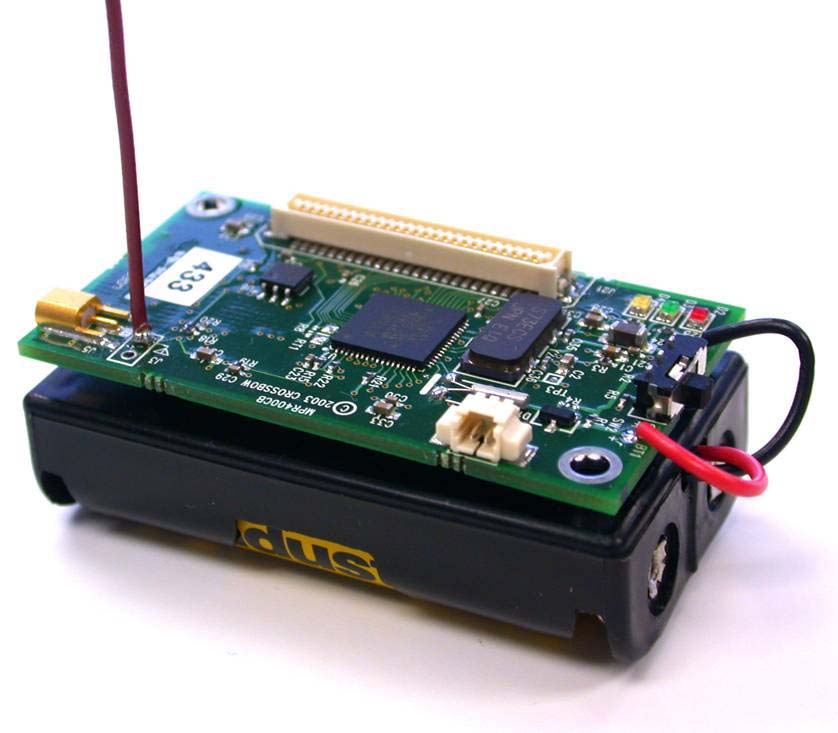
\includegraphics[width=0.6\textwidth]{mica2}~\\[1cm]

{ \huge \bfseries Actieve Evacuatie met gebruik van Wireless Sensor Networks \\[0.4cm] }
\hrule
\hspace{0pt} \\[1.3cm]

\begin{minipage}{0.4\textwidth}
\begin{flushleft} \large
\emph{Author:}\\
Roy \textsc{Scheefhals}\\
\emph{Hogeschool Utrecht}\\
Studentnummer: 1563303\\
\end{flushleft}
\end{minipage}
\begin{minipage}{0.4\textwidth}
\begin{flushright} \large
\emph{Bedrijfsbegeleider:} \\
Martin \textsc{Klomp}\\
\emph{Alten PTS}
\end{flushright}
\end{minipage}

\end{center}
\end{titlepage}

\thispagestyle{empty}
\renewcommand{\thesection}{\Roman{section}}

\section*{Versiebeheer}
\begin{tabular}{ | l | l | l | p{7.5cm} |}
\hline
Versie & Wanneer & Wat \\ \hline
0.1 & 05-03-2014 & Eerste opzet document\\ \hline
0.2 & 07-03-2014 & Achtergrond Project v1\\ \hline
1.0 & 31-03-2014 & Eerste versie\\ \hline

\end{tabular}

\clearpage\pagenumbering{roman}

\chapter{Inleiding}
\subfile{Inleiding}

\newpage\pagenumbering{arabic}
\renewcommand{\thesection}{\arabic{section}}
\renewcommand*\contentsname{Inhoud}
\setlength{\cftbeforetoctitleskip}{-3em}
\tableofcontents

\clearpage

\chapter{Achtergrond van Project} 
\subfile{Achtergrond}

\chapter{Project Definitie}
\subfile{Opdracht}

\chapter{Planning en Aanpak}
\subfile{Planning-aanpak}

\bibliographystyle{plain}
\bibliography{mybib}

\subfile{Bijlagen}


\end{document}
